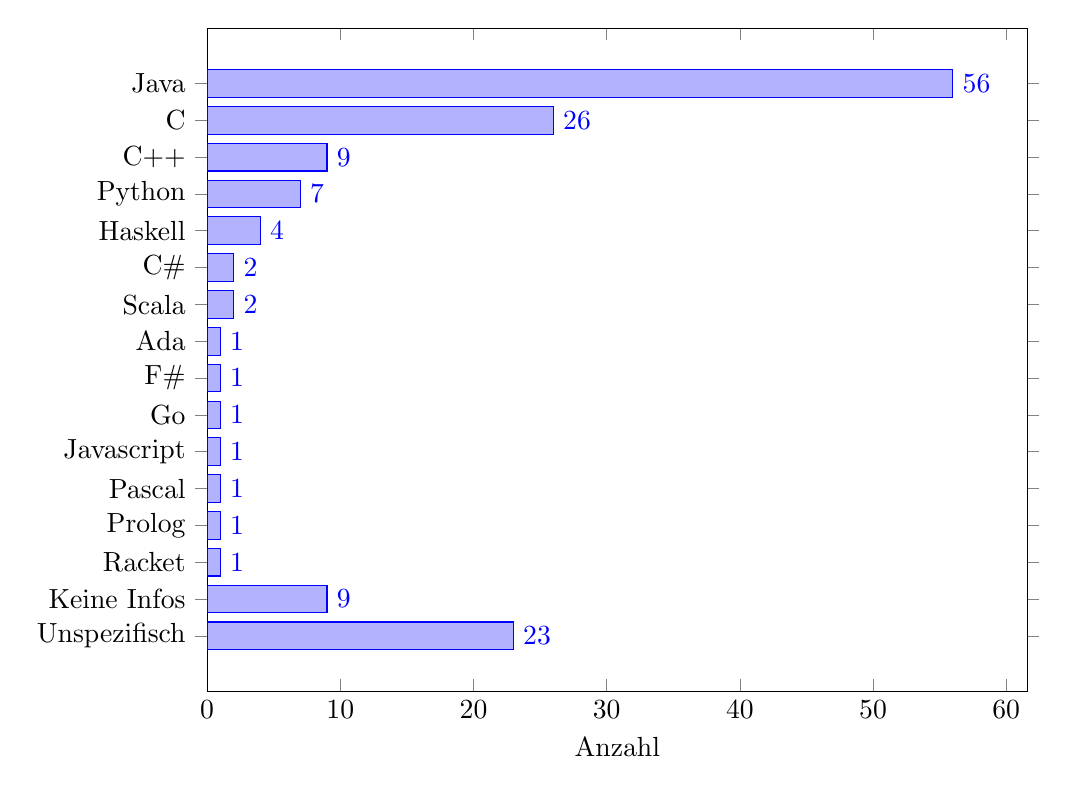
\begin{tikzpicture}
    \begin{axis}[
        xbar,
        width=12cm,
        height=10cm,
        symbolic y coords={{Unspezifisch}, {Keine Infos}, {Racket}, {Prolog}, {Pascal}, {Javascript}, {Go}, {F\#}, {Ada}, {Scala}, {C\#}, {Haskell}, {Python}, {C++},  {C}, {Java}},
        ytick=data,
        nodes near coords,
        xmin=0,
        xlabel={Anzahl}
    ]
        \addplot coordinates {
            (23,{Unspezifisch}) (9,{Keine Infos}) (1,{Racket}) (1,{Prolog}) (1,{Pascal}) (1,{Javascript}) (1,{Go}) (1,{F\#}) (1,{Ada}) (2,{Scala}) (2,{C\#}) (4,{Haskell}) (7,{Python})  (9,{C++}) (26,{C}) (56,{Java})
        };
    \end{axis}
\end{tikzpicture}
